\subsubsubsubsection{UEDirector}
\begin{figure}[h]
\centering
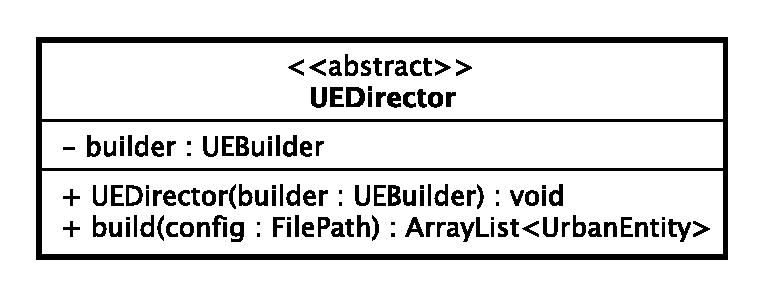
\includegraphics[scale=0.6,keepaspectratio]{images/solution/uedirector.eps}
\caption{App::Reactive::UEDirector}
\label{fig:sd-app-uedirector}
\end{figure}
\FloatBarrier
\begin{itemize}
  \item \textbf{Description} \\
    It represents the urban entity director which instructs the builder.
  \item \textbf{Attribute}
  \begin{itemize}
    \item \texttt{- builder: UEBuilder} \\
The builder object which builds parts of the district.
  \end{itemize}
  \item \textbf{Operation}
  \begin{itemize} 
    \item \texttt{+ UEDirector(builder: UEBuilder)} \\
Creates a director with its own builder object.
    \item \texttt{+ build(config: FilePath) : ArrayList<UrbanEntity>} \\
Builds a list of urban entities according to the configuration file. It uses the
builder multiple times to create incrementally a configuration of the requested
urban entity as specified in the configuration file.
  \end{itemize}
\end{itemize}
